% !TEX root = ../main.tex
\chapter{Matematiske verktøy vi trenger}
\label{Chapter:matematikk}
\intro{I fysikk bruker vi matematikken som et presist språk for å beskrive verden rundt oss. Her ser vi på de viktigste matematiske verktøyene du trenger i dette kurset. Det betyr ikke at vi går nøye gjennom alt, men kapitlet gir en oversikt over de grunnleggende konseptene og reglene du bør være komfortabel med.}
\tanke{}{%
Hvorfor kan naturen beskrives med matematikk?}

\begin{mymerk*}{Python og programmering}
I dette kompendiet bruker vi Python for å illustrere beregninger og lage figurer. Om du aldri har programmert før, anbefaler vi å lese Appendiks~\ref{app:python} før du går videre. Der finner du en kort innføring i alt du trenger for å komme i gang.
\end{mymerk*}

\section{Likninger og algebra}

Likninger handler om å uttrykke sammenhenger mellom størrelser ved hjelp av variabler og symboler. I stedet for å skrive at «fart er strekning delt på tid» kan vi skrive
\[
v = \frac{s}{t}.
\]
Her er $v$, $s$ og $t$ \emph{variabler} — altså symboler som kan ta ulike tallverdier. 

Noe av det vi kommer til å gjøre mest i fysikken er å sette opp likninger og løse for en variabel; en såkalt "ukjent". Da må vi følge gitte logiske regler. Disse reglene kalles algebra-regler, eller bare algebra.

\exm{Finne gjennomsnittsfart $\bar{v}$}{Jakob Ingebrigtsen er ute og løper. Han løper $s_1 = \SI{5}{\kilo\metre}$ på $t_1 = \SI{20}{\minute}$. Deretter skrur han opp tempo litt og løper en strekning $s_2 = \SI{4}{\kilo\metre}$ på $t_2 = \SI{18}{\minute}$. Hva er gjennomsnittsfarten $\bar{v}$?

\paragraph{Løsning:} Gjennomsnittsfart $\bar{v}$ er også et begrep vi ikke har lært ennå, men det er rett fram, og de fleste kjenner det intuitivt igjen fra erfaring:
\[\hat{v} = \frac{\text{total strekning}}{\text{total tid}}.\]
Vi må derfor finne total strekning og total tid før vi kan regne ut gjennomsnittsfarten.

Først finner vi total strekning og total tid:
\[
s_{\text{total}} = s_1 + s_2 = \SI{5}{\kilo\metre} + \SI{4}{\kilo\metre} = \SI{9}{\kilo\metre},
\]
\[
t_{\text{total}} = t_1 + t_2 = \SI{20}{\minute} + \SI{18}{\minute} = \SI{38}{\minute}.
\]
Gjennomsnittsfarten er da:
\[
\bar{v} = \frac{s_{\text{total}}}{t_{\text{total}}} = \frac{\SI{9}{\kilo\metre}}{\SI{38}{\minute}} = \doubleunderline{\SI{0.237}{\kilo\metre\per\minute}} = 0.237\cdot\frac{\SI{1\,000}{\metre}}{\SI{60}{\second}} = \doubleunderline{\SI{3.95}{\metre\per\second}}.
\]
Greier du å gjøre dette om til km/t?

}
Et annet eksempel kan være Newtons 2. lov, som gir sammenhengen mellom det vi kaller for kraft $F$, masse $m$ og akselerasjon $a$. 


\exm{Løse for akselerasjon $a$}{Newtons 2. lov sier $F = m \cdot a$. En bil med masse $m = \SI{1\,200}{\kilo\gram}$ utsettes for en kraft $F = \SI{4\,800}{\newton}$. Finn akselerasjonen $a$.

\paragraph{Løsning:} Del begge sider på $m$:
\[
a = \frac{F}{m} = \frac{\SI{4\,800}{\newton}}{\SI{1\,200}{\kilo\gram}} = \doubleunderline{\SI{4.0}{\metre\per\second\squared}}.
\]
}

\paragraph{Python som kalkulator: } I dette faget er ikke Python obligatorisk, men dere kommer nok til å trenge det i mange andre fag, så det er greit å bli vant med det først som sist. La oss starte med å se et eksempe hvor vi enkelt og greit bruker Python til å utføre noe vi kunne gjort på en gammeldags kalkulator. 
\exm{Kinetisk energi}{%
Beregn den kinetiske energien $E_K=\frac{1}{2}mv^2$ til en gjenstand med masse $m = \SI{2.0}{\kilo\gram}$ som beveger seg med fart $v = \SI{5.0}{\metre\per\second}$.
\paragraph{Løsning:} Vi bruker Python som kalkulator og definerer variablene $m$ og $v$, som vist i koden under.
}
\begin{pythonkode}
# Kinetisk energi: E_k = 0.5 * m * v**2
m = 2.0    # masse i kg
v = 5.0    # fart i m/s

E_k = 0.5 * m * v**2

print(f"Kinetisk energi: {E_k} J")
\end{pythonkode}
\begin{pythonoutput}
Kinetisk energi: 25.0 J
\end{pythonoutput}
\pyfile{TRES0312 Python/Kap2\_MatematiskeVerktoyViTrenger/K2\_algebra\_beregning.ipynb}{Kap2_MatematiskeVerktoyViTrenger/K2_algebra_beregning.ipynb}

\begin{mymerk*}{Kjøre koden selv}
Alle kodeeksempler finnes som Jupyter Notebook-filer i mappen \pyfolderlink. Se Appendiks~\ref{app:python} for hvordan du åpner og kjører dem.
\end{mymerk*}

\oppgave{Algebra og Python}{%
\begin{enumerate}[a)]
    \item Beregn $\dfrac{15 + 3^2}{6 - 2}$ for hånd, og sjekk svaret med Python, eller kalkulator.
    \item Bruk Python (eller en kalkulator) til å beregne potensiell energi $E_p = m \cdot g \cdot h$ for $m = \SI{5.0}{\kilo\gram}$, $g = \SI{9.81}{\metre\per\second\squared}$ og $h = \SI{10.0}{\metre}$.
\end{enumerate}
}
\begin{mymerk*}{}
Om du ikke kjenner til formlene vi her har brukt, som $F=ma$, $E_K = \frac{1}{2}mv^2$ og $E_p = mgh$, så er det ikke noe problem. Vi kommer tilbake til det i senere kapitler. Det viktigste akkurat nå er at du har kontroll på algebaraen.
\end{mymerk*}
Det aller viktiste så langt er at du forstår at fysikkens språk er matematikk, og at vi derfor skriver ned likninger som beskriver sammenhenger mellom størrelser. Vi kan da løse for en ukjent ved å bruke algebra-regler.
\begin{myoppsum*}{Algebraregler}
    \begin{itemize}
        \item Det du gjør på ett ledd i en likningmå du gjøre på alle ledd.
        \item Husk at du alltid kan multiplisere med 1.
    \end{itemize}
\end{myoppsum*}
Det kan også være verdt å repetere følgende regler for notasjon:
\begin{itemize}
    \item \textbf{Potenser:} $x^a \cdot x^b = x^{a+b}$, \quad $\dfrac{x^a}{x^b} = x^{a-b}$, \quad $(x^a)^b = x^{ab}$.
    \item \textbf{Kvadratrot:} $\sqrt{x} = x^{1/2}$.
\end{itemize}
\graabox{I tillegg har vi kvadratsetningene:
\begin{align*}
    &(a+b)^2 = a^2 + 2ab + b^2, \\
    &(a-b)^2 = a^2 - 2ab + b^2, \\
    &(a+b)(a-b) = a^2 - b^2.
\end{align*}}
Disse bør også sitte i fingrene.

\section{Funksjoner og plotting}

En \emph{funksjon} er en regel som til enhver innverdi $x$ knytter én bestemt utverdi $f(x)$. I fysikk er funksjoner et sentralt verktøy — for eksempel er posisjonen $s$ til et objekt i bevegelse en funksjon av tid $t$. Da skriver vi gjerne $s(t)$ som funksjonsnavn. 

\subsection*{Lineær funksjon}
Den enkleste funksjonen er den lineære:
\graabox{$\displaystyle f(x) = b + ax$}
der $a$ er \emph{stigningstallet} (hvor bratt grafen er) og $b$ er \emph{konstantleddet} (der grafen skjærer $y$-aksen). Et slikt eksempel er farten $v(t)$ når akselerasjonen er konstant: \[v(t) = v_0 + at.\]
Som du ser så bruker vi forskjellige variabelnavn, avhengig av hva vi prater om. Det er viktig å forstå at variabelnavnene i seg selv ikke er viktige. Vi kunne i prinsippet godt ha kalt fartsfunksjonen for $f(t)$, uten at det hadde endret noe som helst. Det er bare ikke så hensiktsmessig. 

\subsection*{Kvadratisk funksjon}
En kvadratisk funksjon har formen
\graabox{$\displaystyle f(x) = ax^2 + bx + c$}
Grafen er en parabel. Posisjonen til et legeme med konstant akselerasjon er for eksempel en kvadratisk funksjon av tid:
\[s(t) = \frac{1}{2}at^2+ v_0 t + s_0.\]

\begin{mymerk*}{}
Merk at mange bokstaver kan symbolisere veldig forskjellige ting. Bokstaven $s$ er et godt eksempel. Skriver vi $s(t)$ mener vi nok strekning som funksjon av tid $t$. Men tiden $t$ har jo enhet sekund, som også betegnes med bokstaven $s$! Et annet eksempel er bokstaven $m$, som brukes både til å symbolisere masse, men også som symbol for enheten meter. Ut ifra sammenhengen greier man som regel å forstå hva som er ment — i alle fall med litt trening.
\end{mymerk*}
\subsection*{Plotting med Python}
En av de nyttigste tingene vi kan gjøre med Python, er å tegne grafer. Eksemplet under plotter posisjon og fart som funksjon av tid for et legeme med konstant akselerasjon:

\begin{pythonkode}
import numpy as np
import matplotlib.pyplot as plt

# Parametre
a  = 2.0    # akselerasjon [m/s^2]
v0 = 0.0    # startfart [m/s]
s0 = 0.0    # startposisjon [m]

# Tid fra 0 til 5 sekunder (200 punkter)
t = np.linspace(0, 5, 200)

# Bevegelsesligninger
s = s0 + v0*t + 0.5*a*t**2   # posisjon
v = v0 + a*t                  # fart

# To grafer side om side
fig, (ax1, ax2) = plt.subplots(1, 2, figsize=(10, 4))

ax1.plot(t, s, color='royalblue', linewidth=2)
ax1.set_xlabel('Tid [s]')
ax1.set_ylabel('Posisjon [m]')
ax1.set_title('Posisjon vs. tid')
ax1.grid(True, alpha=0.3)

ax2.plot(t, v, color='tomato', linewidth=2)
ax2.set_xlabel('Tid [s]')
ax2.set_ylabel('Fart [m/s]')
ax2.set_title('Fart vs. tid')
ax2.grid(True, alpha=0.3)

plt.tight_layout()
plt.show()
\end{pythonkode}
\pyfile{TRES0312 Python/Kap2\_MatematiskeVerktoyViTrenger/K2\_funksjoner\_og\_plotting.ipynb}{Kap2_MatematiskeVerktoyViTrenger/K2_funksjoner_og_plotting.ipynb}
\begin{figure}[H]
\centering
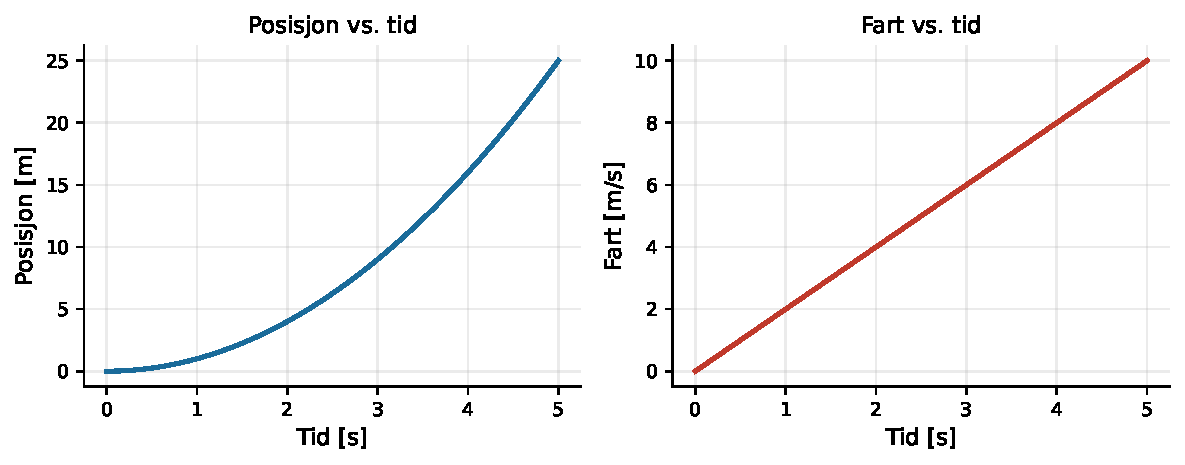
\includegraphics[width=0.95\linewidth]{Images/Kapittel1:introduksjon/python_plot_02_bevegelse.pdf}
\caption{Posisjon og fart som funksjon av tid for konstant akselerasjon $a=\SI{2.0}{\metre\per\second\squared}$, $v_0 = 0$.}
\end{figure}

\oppgave{Funksjoner og plotting}{%
\begin{enumerate}[a)]
    \item Bruk Python (eller et annet verktøy du måtte foretrekke) til å plotte funksjonen $f(x) = 2x^2 - 3x + 1$ for $x \in [-2,\, 4]$.
    \item Modifiser Python-koden gitt i teksten over slik at startfarten er $v_0 = \SI{3.0}{\metre\per\second}$. Hva forandrer seg i grafene? Grafen du plotter i oppgave a) kan være til hjelp for å se svaret.
\end{enumerate}
}

\section{Trigonometri}

Trigonometri er veldig nyttig redskap i fysikken, ettersom vi hele veien har bruk for å dekomponere vektorer i koordinatsystem. Det er antatt at studentene kjenner dette begrepsaparatet fra før, men her følger en liten oppsummering.

\paragraph{I en rettvinklet trekant} navngir vi sidene i forhold til en valgt vinkel $\theta$:
\begin{itemize}
    \item \textbf{Hypotenus} ($c$) — den lengste siden, alltid overfor den rette vinkelen ($90-$graders vinkelen). Denen sidekanten vil utgjøre det ene benet ivinkelen $\theta$.
    \item \textbf{Hosliggende katet} (a) — sidekanten som utgjør det andre benet i $\theta$-vinkelen.
    \item \textbf{Motstående katet} (b) — siden overfor $\theta$
\end{itemize}

\noindent\begin{minipage}{\linewidth}
\begin{center}
\begin{tikzpicture}[scale=1.25, baseline=(current bounding box.center)]
  \coordinate (O) at (0,0);
  \coordinate (A) at (3.2,0);
  \coordinate (B) at (3.2,2);
  \fill[headCol!9] (O) -- (A) -- (B) -- cycle;
  \draw[thick] (O) -- (A) node[midway, below=6pt] {\small hosliggende ($a$)};
  \draw[thick] (A) -- (B) node[midway, right=5pt] {\small motstående ($b$)};
  \draw[thick] (O) -- (B) node[midway, above left=2pt] {\small hypotenus ($c$)};
  \draw (A) ++(-0.22,0) -- ++(0,0.22) -- ++(0.22,0);
  \draw[headCol, thick] (0.55,0) arc (0:32:0.55);
  \node at (0.84,0.14) {$\theta$};
\end{tikzpicture}
\hspace{2.5cm}
\begin{tikzpicture}[scale=1.6, baseline=(current bounding box.center)]
  \draw[->] (-1.2,0) -- (1.3,0) node[right, font=\small] {$x$};
  \draw[->] (0,-1.2) -- (0,1.3) node[above, font=\small] {$y$};
  \draw[thick] (0,0) circle (1);
  \fill[headCol] (0.707,0.707) circle (1.8pt);
  \draw[thick, headCol] (0,0) -- (0.707,0.707)
        node[midway, above left=1pt, font=\small] {$1$};
  \draw[dashed, gray!60] (0.707,0) -- (0.707,0.707);
  \draw[dashed, gray!60] (0,0.707) -- (0.707,0.707);
  \draw[very thick, thmscol] (0,0) -- (0.707,0)
        node[midway, below=4pt, font=\small] {$\cos\theta$};
  \draw[very thick, defscol!80!black] (0,0) -- (0,0.707)
        node[midway, left=4pt, font=\small] {$\sin\theta$};
  \draw[->] (0.28,0) arc (0:45:0.28);
  \node[font=\small] at (0.45,0.13) {$\theta$};
  \node[font=\small, above right=1pt] at (0.707,0.707) {$P$};
\end{tikzpicture}
\end{center}
\begin{center}
\small\textit{Venstre: rettvinklet trekant med vinkel $\theta$. \quad Høyre: enhetssirkelen ($r=1$), der $P=(\cos\theta,\,\sin\theta)$.}
\end{center}
\end{minipage}

Pythagoras læresetning sier nå at 
\begin{align*}
    a^2 + b^2 = c^2.
\end{align*}
Vi kan nå definere de trigonometriske funksjonene sinus, cosinus og tangens.
\defn{Sinus, cosinus og tangens}{For en vinkel $\theta$ i en rettvinklet trekant med hypotenus $c$ har vi nå følgende definisjoner:
\begin{align*}
    \cos\theta = \frac{\text{hosligg.}}{\text{hyp.}}=\frac{a}{c}, \qquad
    \sin\theta = \frac{\text{motst.}}{\text{hyp.}}=\frac{b}{c}, \qquad
    \tan\theta = \frac{\sin\theta}{\cos\theta} = \frac{\text{motst.}}{\text{hosligg.}}=\frac{b}{a}.
\end{align*}
}
Ut ifra formlene over så se vi at vi får følgende formlerfor katetene $a$ og $b$:
\[
\text{a} = c\cos\theta, \qquad \text{b} = c\sin\theta.
\]
Dette er uttrykk som vi kommer til å benytte oss av veldig mye. Jeg anbefaler å pugge uttrykkene i den grønne boksen, og alltid utlede ting på nytt derifra når du trenger det.

\paragraph{Enhetssirkelen} er et veldig nyttig verktøy når man jobber med trigonometriske funksjoner. Enhetssirklene er rett og slett en sirkel med radius 1, slik at katetene i trekanten med vinkel $\theta$ skrevet inn i enhetssirkelen, blir $\cos\theta$ og $\sin\theta$. Da ser vi også umiddelbart fra Pythagoras læesetning at 
\begin{align*}
    \cos^2\theta + \sin^2\theta = 1.
\end{align*}
Denne formelen er mye brukt, så den kan du bare lære deg med det samme. Tabellen under viser noen eksakte verdier for de trigonometriske funksjonene. De fleste vinklene har ikke eksakte uttrykk på denne formen, men disse er mye brukte vinkler, og det kan derfor være kjekt å kjenne til dem. Jeg anbefaler likevel ikke å bruke tid på å pugge de.

\begin{table}[H]
\centering
\renewcommand{\arraystretch}{1.55}
\begin{tabular}{|c|c|c|c|}
\hline
\rowcolor{blue!20!black!10}
$\theta$ & $\sin\theta$ & $\cos\theta$ & $\tan\theta$ \\
\hline
$0^\circ$  & $0$ & $1$ & $0$ \\
\hline
$30^\circ$ & $\dfrac{1}{2}$ & $\dfrac{\sqrt{3}}{2}$ & $\dfrac{1}{\sqrt{3}}$ \\
\hline
$45^\circ$ & $\dfrac{\sqrt{2}}{2}$ & $\dfrac{\sqrt{2}}{2}$ & $1$ \\
\hline
$60^\circ$ & $\dfrac{\sqrt{3}}{2}$ & $\dfrac{1}{2}$ & $\sqrt{3}$ \\
\hline
$90^\circ$ & $1$ & $0$ & — \\
\hline
\end{tabular}
\caption{Viktige trigonometriske verdier.}
\label{tab:trig}
\end{table}

\exm{Trigonometri: stige mot vegg}{En stige av lengde $h = \SI{5.0}{\metre}$ lener seg mot en vegg i vinkel $\theta = 37^\circ$ med gulvet. Finn den horisontale og vertikale komponenten til stigen.

\paragraph{Løsning:}
\begin{align*}
x &= h\cos\theta = 5.0\cdot\cos 37^\circ \approx 5.0\cdot 0.799 \approx \doubleunderline{\SI{4.0}{\metre}} \\
y &= h\sin\theta = 5.0\cdot\sin 37^\circ \approx 5.0\cdot 0.602 \approx \doubleunderline{\SI{3.0}{\metre}}
\end{align*}
Dette er nøyaktig et $(3,4,5)$-trekant skalert med $\SI{1}{\metre}$.
}

\exm{Bruk av $\sin^2\theta + \cos^2\theta = 1$}{En vinkel $\theta$ i første kvadrant har $\sin\theta = \dfrac{3}{5}$.
\begin{enumerate}[a)]
    \item Bruk sammenhengen $\sin^2\theta + \cos^2\theta = 1$ til å finne $\cos\theta$.
    \item Finn $\tan\theta$.
\end{enumerate}

\paragraph{Løsning:}
\paragraph{a)} Vi løser for $\cos\theta$:
\[
\cos^2\theta = 1 - \sin^2\theta = 1 - \left(\frac{3}{5}\right)^2 = 1 - \frac{9}{25} = \frac{16}{25}.
\]
Siden $\theta$ er i første kvadrant er $\cos\theta$ positiv, så
\[
\cos\theta = \sqrt{\frac{16}{25}} = \doubleunderline{\frac{4}{5}}.
\]
\paragraph{b)}
\[
\tan\theta = \frac{\sin\theta}{\cos\theta} = \frac{3/5}{4/5} = \doubleunderline{\frac{3}{4}}.
\]
}

\exm{Fortegn til $\sin\theta$ og $\cos\theta$}{Bruk enhetssirkelen til å avgjøre om $\sin\theta$ og $\cos\theta$ er positiv eller negativ for hver av vinklene:
\begin{enumerate}[a)]
    \item $\theta = 120^\circ$
    \item $\theta = 200^\circ$
    \item $\theta = 300^\circ$
\end{enumerate}
I hvilken kvadrant er både $\sin\theta$ og $\cos\theta$ positive? I hvilken kvadrant er begge negative?

\paragraph{Løsning:} På enhetssirkelen er $\cos\theta$ lik $x$-koordinaten og $\sin\theta$ lik $y$-koordinaten til punktet på sirkelen. Fortegnet avhenger derfor av hvilken kvadrant vinkelen $\theta$ befinner seg i.
\paragraph{a)} $\theta = 120^\circ$ ligger i andre kvadrant ($90^\circ < \theta < 180^\circ$), der $x<0$ og $y>0$: \doubleunderline{$\sin\theta$ positiv, $\cos\theta$ negativ.}
\paragraph{b)} $\theta = 200^\circ$ ligger i tredje kvadrant ($180^\circ < \theta < 270^\circ$), der $x<0$ og $y<0$: \doubleunderline{$\sin\theta$ negativ, $\cos\theta$ negativ.}
\paragraph{c)} $\theta = 300^\circ$ ligger i fjerde kvadrant ($270^\circ < \theta < 360^\circ$), der $x>0$ og $y<0$: \doubleunderline{$\sin\theta$ negativ, $\cos\theta$ positiv.}

Begge er positive i \doubleunderline{første kvadrant} ($0^\circ < \theta < 90^\circ$), og begge er negative i \doubleunderline{tredje kvadrant} ($180^\circ < \theta < 270^\circ$).
}

\oppgave{Trigonometri}{%
\begin{enumerate}[a)]
    \item Les av $\sin 30^\circ$, $\cos 45^\circ$ og $\tan 60^\circ$ fra Tabell~\ref{tab:trig}.
    \item En trekant har hypotenus $c = \SI{10}{\metre}$ og vinkel $\theta = 53^\circ$. Finn lengden av den motstående kateten $b$ og den hosliggende kateten $a$.
    \item Vis at $\sin^2 30^\circ + \cos^2 30^\circ = 1$.
    \item Hva blir $(\sin\theta+1)(\sin\theta-1)$? Hint: Bruk en av kvadratsetningene.
\end{enumerate}
}

\section{Vektorer}
Vektorer kan sees på som utvidelse av tall til flere dimensjoner. Vi får da et objekt som med vår bruk kan representeres som en pil i et koordinatsystem. Vi kan gå så langt som å si at det er dette vektorer er for oss.

\defn{vektor}{En vektor er et matematisk objekt med både størrelse og retning. Vi bruker en pil for å si at det er en vektor: $\vec{A}.$}
Det vi tidligere kalte tall, refererer vi nå gjerne til som \textit{skalarer}, altså ikke vektorer. Skalarer har kun størrelse, og ikke retning. Det neste vi må gjøre er å definere hva vi mener med operasjoner som addisjon ($+$) og multiplikasjon ($\cdot$) for vektorer. 

\noindent\begin{minipage}{\linewidth}
\begin{center}
\begin{tikzpicture}[scale=1.0, baseline=(current bounding box.center)]
  %--- Frie vektorer A og B (ingen koordinatsystem) ---
  % Vektor A
  \draw[->, thick, headCol] (0,0.7) -- (2.4,1.5);
  \node[above=2pt, font=\small, headCol] at (1.2,1.1) {$\vec{A}$};
  % Pluss-tegn
  \node[font=\large] at (2.85,1.1) {$+$};
  % Vektor B
  \draw[->, thick, defscol!80!black] (3.3,0.35) -- (4.0,1.75);
  \node[right=3pt, font=\small, defscol!80!black] at (3.65,1.05) {$\vec{B}$};
\end{tikzpicture}
\hspace{2cm}
\begin{tikzpicture}[scale=1.0, baseline=(current bounding box.center)]
  %--- Tip-til-hale-addisjon: C = A + B ---
  % Vektor A fra origo
  \draw[->, thick, headCol] (0,0) -- (2.4,0.8);
  \node[below=3pt, font=\small, headCol] at (1.2,0.4) {$\vec{A}$};
  % Vektor B plassert ved spissen av A
  \draw[->, thick, defscol!80!black] (2.4,0.8) -- (3.1,2.2);
  \node[right=3pt, font=\small, defscol!80!black] at (2.75,1.5) {$\vec{B}$};
  % Resultantvektor C
  \draw[->, very thick, oppgcol] (0,0) -- (3.1,2.2);
  \node[left=4pt, font=\small, oppgcol] at (1.55,1.1) {$\vec{C}$};
\end{tikzpicture}
\end{center}
\begin{center}
  {\small\textit{Venstre: vektorene $\vec{A}$ og $\vec{B}$. \quad
  Høyre: $\vec{B}$ plassert ved spissen av $\vec{A}$ gir resultantvektoren
  $\vec{C} = \vec{A} + \vec{B}$ (tip-til-hale-metoden).}}
\end{center}
\end{minipage}
Multiplikasjon skal vi komme tilbake til litt senere.

\oppgave{Skalarer og vektorer}{%
Er følgende fysiske størrelser skalarer eller vektorer? Begrunn svaret.
\begin{enumerate}[a)]
    \item Temperatur
    \item Posisjon
    \item Fart
    \item Hastighet
    \item Akselerasjon
    \item Masse
\end{enumerate}
}
La oss nå gå over til å introdusere koordinatsystem, som er et viktig verktøy for å kunne regne med vektorer på en effektiv måte i fysikken.
\subsection{Koordinatsystem}
Et koordinatsystem er et verktøy vi bruker for å beskrive posisjon. Dette er helt essensielt i fysikken, for eksempel når vi ønsker å beskrive bevegelse i planet eller rommet.

\noindent\begin{minipage}{\linewidth}
\begin{center}
\begin{tikzpicture}[scale=1.05, baseline=(current bounding box.center)]
  %--- Talllinjen R ---
  \draw[->] (-1.8,0) -- (4.8,0) node[right, font=\small] {$\mathbb{R}$};
  \foreach \x in {-1,0,1,2,3,4} {
    \draw (\x,0.09) -- (\x,-0.09);
    \node[below=3pt, font=\small] at (\x,0) {$\x$};
  }
  \fill[headCol] (3,0) circle (2.5pt);
  \node[above=5pt, font=\small, headCol] at (3,0) {$P = 3$};
\end{tikzpicture}
\hspace{2.5cm}
\begin{tikzpicture}[scale=0.95, baseline=(current bounding box.center)]
  %--- Koordinatsystemet R^2 ---
  \draw[->] (-0.5,0) -- (4.6,0) node[right, font=\small] {$x$};
  \draw[->] (0,-0.5) -- (0,3.4) node[above, font=\small] {$y$};
  \foreach \x in {1,2,3,4} {
    \draw (\x,0.08) -- (\x,-0.08);
    \node[below=3pt, font=\small] at (\x,0) {$\x$};
  }
  \foreach \y in {1,2,3} {
    \draw (0.08,\y) -- (-0.08,\y);
    \node[left=3pt, font=\small] at (0,\y) {$\y$};
  }
  \draw[dashed, gray!60] (3,0) -- (3,2) -- (0,2);
  \fill[headCol] (3,2) circle (2.5pt);
  \node[above right=2pt, font=\small, headCol] at (3,2) {$P = (3,\,2)$};
\end{tikzpicture}
\end{center}
\begin{center}
  {\small\textit{Venstre: tallinjen $\mathbb{R}$ med punkt $P=3$.
  \quad Høyre: planet $\mathbb{R}^2$ med punkt $P=(3,\,2)$.
  Stiplete linjer markerer koordinatene.}}
\end{center}
\end{minipage}

\medskip

\noindent\begin{minipage}{\linewidth}
\begin{center}
\begin{tikzpicture}[scale=1.05, baseline=(current bounding box.center)]
  %--- Talllinjen med posisjonsvektor ---
  \draw[->] (-1.8,0) -- (4.8,0) node[right, font=\small] {$\mathbb{R}$};
  \foreach \x in {-1,0,1,2,3,4} {
    \draw (\x,0.09) -- (\x,-0.09);
    \node[below=3pt, font=\small] at (\x,0) {$\x$};
  }
  \draw[->, very thick, headCol] (0,0) -- (3,0);
  \fill[headCol] (3,0) circle (2.5pt);
  \node[above=5pt, font=\small, headCol] at (3,0) {$P$};
  \node[above=14pt, font=\small, headCol] at (1.5,0) {$r = 3$};
\end{tikzpicture}
\hspace{2.5cm}
\begin{tikzpicture}[scale=0.95, baseline=(current bounding box.center)]
  %--- Koordinatsystemet med posisjonsvektor ---
  \draw[->] (-0.5,0) -- (4.6,0) node[right, font=\small] {$x$};
  \draw[->] (0,-0.5) -- (0,3.4) node[above, font=\small] {$y$};
  \foreach \x in {1,2,3,4} {
    \draw (\x,0.08) -- (\x,-0.08);
    \node[below=3pt, font=\small] at (\x,0) {$\x$};
  }
  \foreach \y in {1,2,3} {
    \draw (0.08,\y) -- (-0.08,\y);
    \node[left=3pt, font=\small] at (0,\y) {$\y$};
  }
  \draw[dashed, gray!60] (3,0) -- (3,2) -- (0,2);
  \draw[->, very thick, headCol] (0,0) -- (3,2);
  \fill[headCol] (3,2) circle (2.5pt);
  \node[above right=2pt, font=\small, headCol] at (3,2) {$P = (3,\,2)$};
  \node[above left=1pt, font=\small, headCol] at (1.55,1.1) {$\vec{r}$};
\end{tikzpicture}
\end{center}
\begin{center}
  {\small\textit{Avstand fra origo til $P$ som vektor:
  $r = 3$ i $\mathbb{R}$ (venstre) og $\vec{r} = (3,\,2)$ i $\mathbb{R}^2$ (høyre).}}
\end{center}
\end{minipage}

I et todimensjonalt koordinatsystem, som $xy$-planet, beskrives en posisjon ved hjelp av et ordnet par $(x,y)$. Her angir:
\begin{itemize}
    \item $x$ posisjonen i horisontal retning
    \item $y$ posisjonen i vertikal retning
\end{itemize}

Punktet $(0,0)$ kalles origo, og fungerer som referansepunkt for alle andre posisjoner i koordinatsystemet.

\oppgave{Koordinatsystem}{%
\begin{enumerate}[a)]
    \item Tegn punktene $A = (2,\,3)$, $B = (-1,\,4)$ og $C = (0,\,-2)$ i et koordinatsystem.
    \item Hvilket kvadrant befinner hvert punkt seg i?
    \item Finn midtpunktet $M$ mellom $A$ og $B$. \textit{Hint: } $M = \left(\frac{x_A + x_B}{2},\, \frac{y_A + y_B}{2}\right)$.
\end{enumerate}
}

\subsection{Enhetsvektorer}

For å arbeide systematisk med vektorer er det nyttig å innføre et sett med faste referansevektorer. Disse kalles \emph{basisvektorer}. Dersom basisvektorene har lengde 1, kaller vi de \emph{enhetsvektorer}. Alle andre vektorer kan uttrykkes som en lineær kombinasjon av basisvektorene. Vi lar gjerne enhetsvektorene peke i retningene til koordinataksene, og kaller de $\hat{\mathbf{x}}$ og $\hat{\mathbf{y}}$ i $xy$-planet. I tre dimensjoner har vi også en enhetsvektor $\hat{\mathbf{z}}$ som peker i $z$-retning.

\defn{Enhetsvektor}{En enhetsvektor er en vektor med lengde 1 som angir en bestemt retning i rommet.}

I $xy$-planet finnes det to enhetsvektorer:
\begin{align}
\hat{\mathbf{x}} = \frac{\vec{x}}{x}=[1,0], \qquad \hat{\mathbf{y}} = \frac{\vec{y}}{y}=[0,1].
\end{align}

Her peker $\hat{\mathbf{x}}$ i positiv $x$-retning, mens $\hat{\mathbf{y}}$ peker i positiv $y$-retning. Sammen danner disse enhetsvektorene grunnlaget for koordinatsystemet.
Merk at $\hat{\mathbf{x}}$ og $\hat{\mathbf{y}}$ er ortonormale, det vil si at de står vinkelrett på hverandre, og at de begge har lengde 1.
\begin{mymerk*}{Alternativ notasjon for enhetsvektorer}
I mange lærebøker brukes symbolene $\mathbf{i}$, $\mathbf{j}$ (og  $\mathbf{k}$ i tre dimensjoner) for de samme enhetsvektorene. I dette kompendiet bruker vi $\hat{\mathbf{x}}$, $\hat{\mathbf{y}}$ (og $\hat{z}$ i tre dimensjoner), da denne notasjonen gjør det umiddelbart tydelig hvilken retning enhetsvektoren peker i.
\end{mymerk*}

Enhver vektor i $xy$-planet kan skrives som en lineær-kombinasjon av enhetsvektorene. Det finnes to ekvivalente skrivemåter:
\begin{align}
\vec{v} = [v_x, v_y] = v_x \hat{\mathbf{x}} + v_y \hat{\mathbf{y}}.
\end{align}

Begge disse skrivemåtene tydeliggjør hvordan vektoren er bygget opp av bidrag i hver retning. Tallene $v_x$ og $v_y$ kalles vektorens komponenter i henholdsvis $x$- og $y$-retning. Prosessen med å finne komponentene til en vektor kalles \emph{dekomponering}, og er tema for neste avsnitt.

\oppgave{Vektorer som en lineærkombinasjon av enhetsvektorer}{%
\begin{enumerate}[a)]
    \item Skriv vektoren $\vec{A} = [4,\,-3]$ som en lineær kombinasjon av enhetsvektorene $\hat{\mathbf{x}}$ og $\hat{\mathbf{y}}$.
    \item Regn ut summen $\vec{u} + \vec{v}$ der $\vec{u} = 3\hat{\mathbf{x}} - 2\hat{\mathbf{y}}$ og $\vec{v} = -\hat{\mathbf{x}} + 5\hat{\mathbf{y}}$. Skriv svaret på komponentform.
\end{enumerate}
}

\subsection{Dekomponering av vektorer i koordinatsystem}
Dekomponering er en generell teknikk i fysikk som innebærer å dele opp en vektor i dens komponenter langs de enkelte koordinataksene\footnote{Eller mer presist langs basisvektorene. Men vi velger disse identisk med koordinataksene, så i praksis blir det ikke noen forskjell. Faktisk kan man si at det å velge et sett med basisvektorer \textit{er} å velge et koordinatsystem. }. Ved å dekomponere en vektor, kan vi forstå hvordan den virker i hver retning separat, noe som gjør komplekse problemer enklere å håndtere. Dette er helt essensielt i alle deler av fysikken som omhandler vektorer. For eksempel, når vi studerer bevegelse i to dimensjoner, som for eksempel en prosjektilbevegelse, slik som vist i Figur~\ref{fig:Prosjektilbevegelse}, så er det veldig nyttig å dekomponere bevegelsen i horisontal og vertikal retning. Da kan vi bruke de enklere bevegelsesligningene for hver retning, og deretter kombinere resultatene for å få en fullstendig beskrivelse av bevegelsen.
\begin{figure}[ht!]
\centering
\begin{tikzpicture}
\node[anchor=south west, inner sep=0] (img) at (0,0)
  {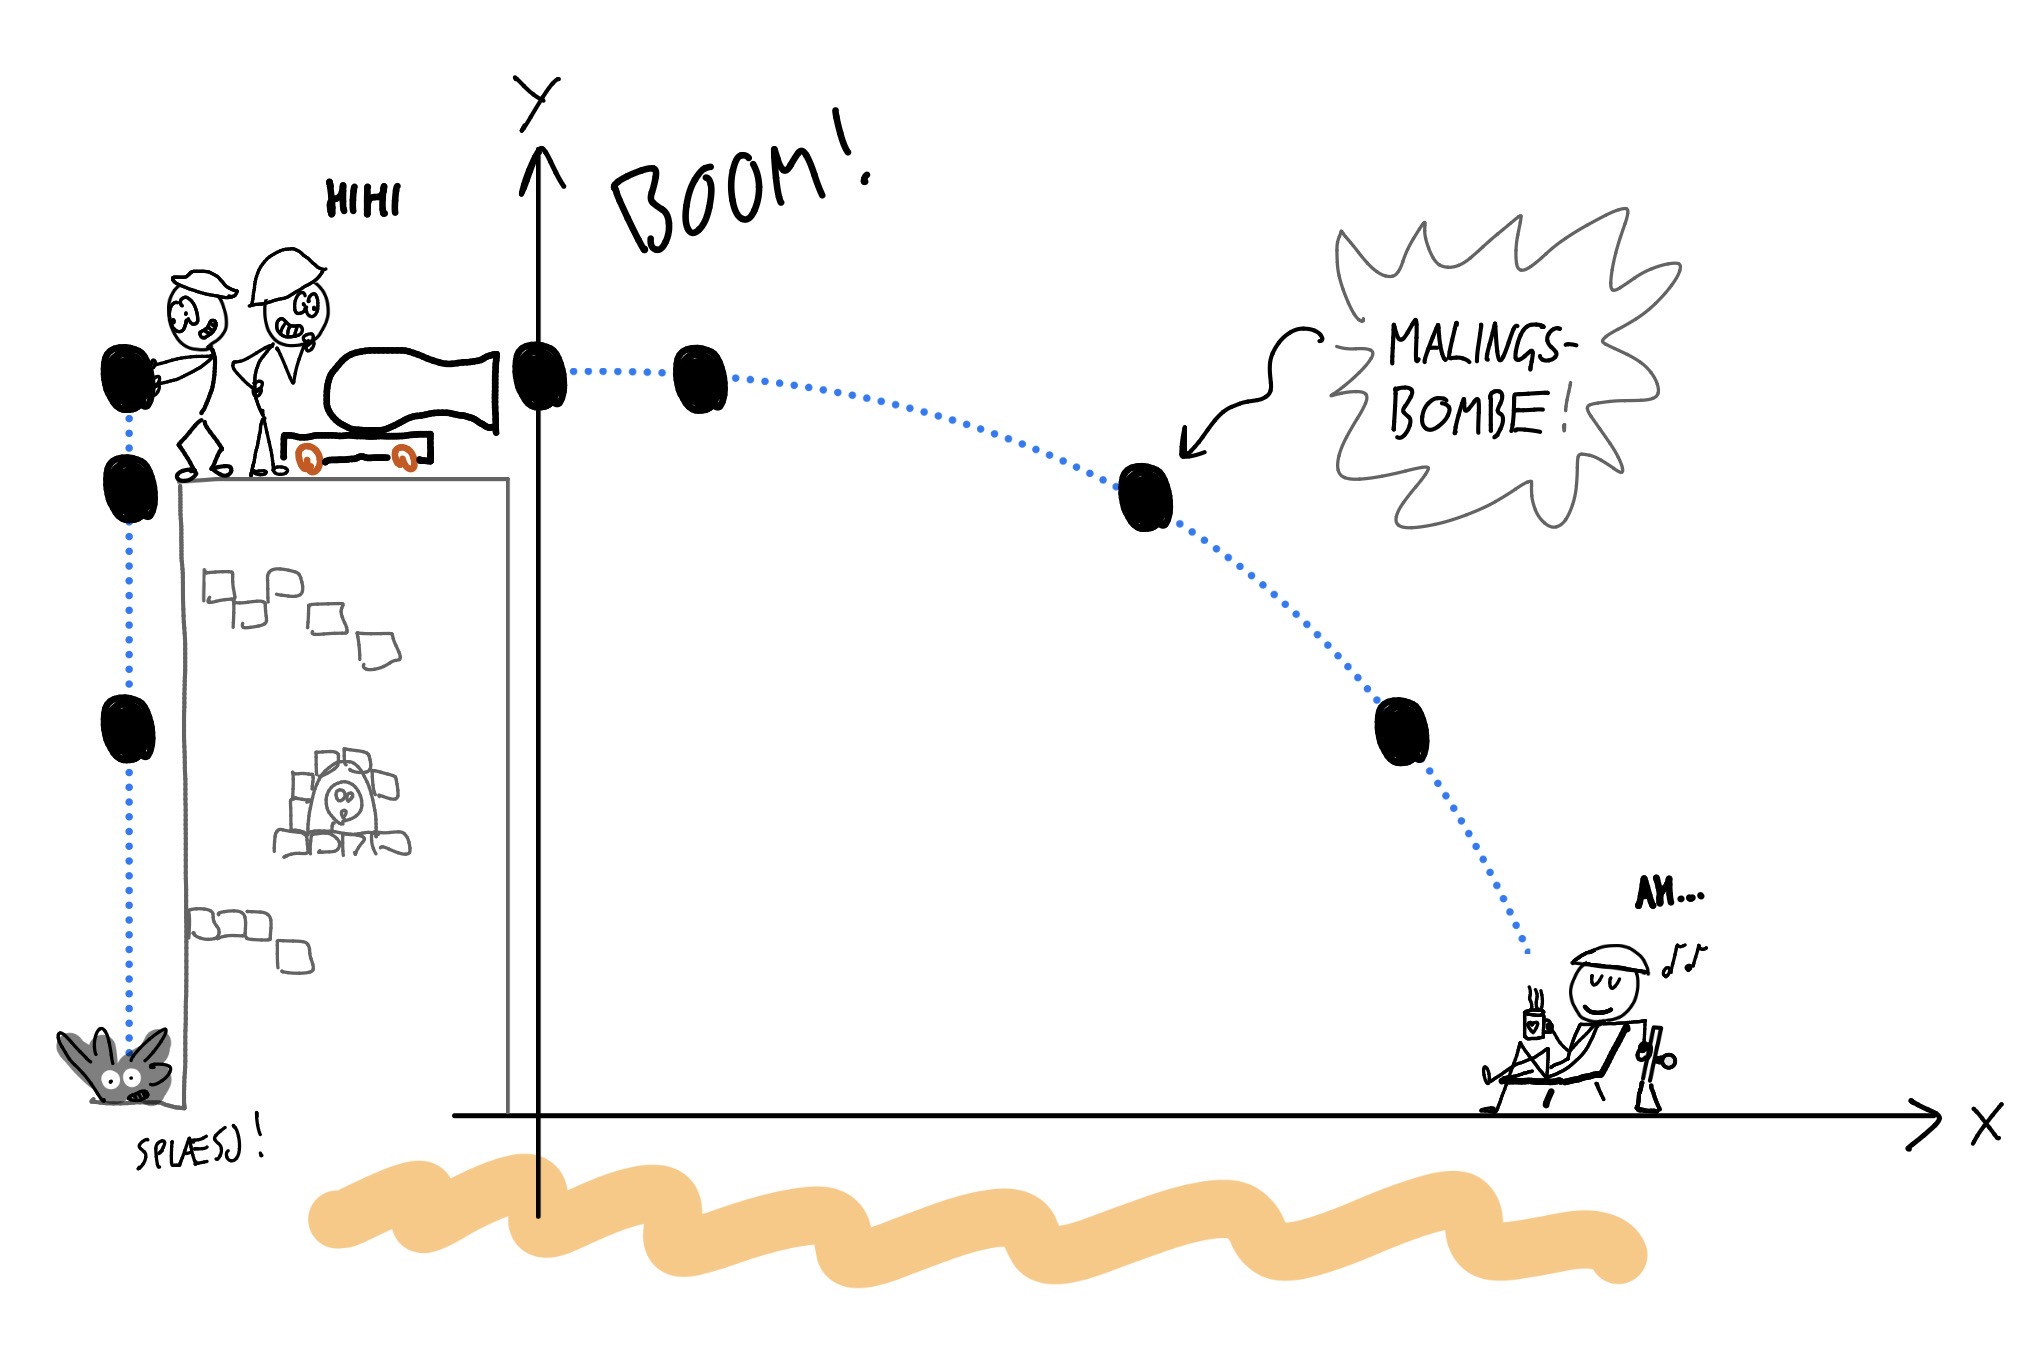
\includegraphics[width=0.8\textwidth]{Images/Kapittel2:Kinematikk/Prosjektilbevegelse_malingsbombe_clean.png}};
\begin{scope}[x={(img.south east)-(img.south west)}, y={(img.north west)-(img.south west)}]
\draw[-{Stealth[length=4mm,width=3mm]}, very thick, headCol] (0.2646,0.1728) -- (0.3443,0.7188);
\draw[-{Stealth[length=4mm,width=3mm]}, very thick, headCol] (0.2646,0.1728) -- (0.5632,0.6313);
\draw[-{Stealth[length=4mm,width=3mm]}, very thick, headCol] (0.2646,0.1728) -- (0.6891,0.4577);
\node[font=\footnotesize, headCol] at (0.3727,0.5094) {$\vec{S}(t_1)$};
\node[font=\footnotesize, headCol] at (0.5044,0.4033) {$\vec{S}(t_2)$};
\node[font=\footnotesize, headCol] at (0.5588,0.2963) {$\vec{S}(t_3)$};
\end{scope}
\end{tikzpicture}
\caption{En malingsbombe i prosjektilbevegelse. Posisjonsvektoren $\vec{S}(t)$ peker fra origo til bomben ved de ulike tidspunktene $t_1$, $t_2$ og $t_3$, og bestemmer dermed banen.}
\label{fig:Prosjektilbevegelse}
\end{figure}

Fysikkens lover formuleres ved hjelp av vektorer, og er uavhengig av valg av koordinatsystem. Likevel innfører vi koordinatsystem når vi saktisk skal regne på noe. Dette er fordi lovene lar seg dekomponere i hver enkelt retning. La oss ta fart som eksempel. Dersom akselerasjonen er konstant så er hastigheten $\vec{v}(t)$ ved tidspunkt $t$ gitt ved starthastigheten $\vec{v}_0$ og akselerasjonen $\vec{a}$ ved formelen
\begin{align}
\vec{v}(t) = \vec{v}_0 + \vec{a}t.
\end{align}
Dette er en vektorlikning, og den gjelder i alle koordinatsystem. Dersom vi velger et koordinatsystem, så kan vi skrive ut komponentene i hver retning, og dermed få to separate likninger:
\begin{align}
v_x(t) = v_{0x} + a_x t, \qquad
v_y(t) = v_{0y} + a_y t.
\end{align}



\exm{Dekomponering av hastighet}{%
En ball kastes med fart $v = \SI{20}{\metre\per\second}$ i en vinkel $\theta = 37°$ over horisonten
($\cos 37° \approx 0{,}80$, $\sin 37° \approx 0{,}60$).\\
\textbf{a)} Finn komponentene $v_x$ og $v_y$.\\
\textbf{b)} Verifiser at $|\vec{v}| = \sqrt{v_x^2 + v_y^2} = \SI{20}{\metre\per\second}$.}

\svar{%
\textbf{a)} Vi bruker de trigonometriske relasjonene $v_x = v\cos\theta$ og $v_y = v\sin\theta$:
\[
v_x = \SI{20}{\metre\per\second}\cdot 0{,}80 = \doubleunderline{\SI{16}{\metre\per\second}},
\qquad
v_y = \SI{20}{\metre\per\second}\cdot 0{,}60 = \doubleunderline{\SI{12}{\metre\per\second}}.
\]
\textbf{b)} Pythagoras bekrefter:
\[
\sqrt{v_x^2 + v_y^2} = \sqrt{(\SI{16}{\metre\per\second})^2 + (\SI{12}{\metre\per\second})^2}
= \sqrt{256 + 144}\,\si{\metre\per\second} = \sqrt{400}\,\si{\metre\per\second} = \doubleunderline{\SI{20}{\metre\per\second}}\;\checkmark
\]
}


\exm{Dekomponering av vektor og beregning av vinkel}{%
Vi har en vektor $\vec{A} = [3,\;4]$ med komponenter $A_x = 3$ og $A_y = 4$.\\
\textbf{a)} Finn størrelsen (skalarverdien) $A = |\vec{A}|$.\\
\textbf{b)} Finn vinkelen $\theta$ mellom $\vec{A}$ og den horisontale aksen.}

\svar{%
\noindent
\begin{minipage}[t]{0.55\linewidth}
  \vspace{0pt}
  \begin{enumerate}[\textbf{a)}]
    \item Størrelsen finner vi med Pythagoras:
          \[A = |\vec{A}| = \sqrt{A_x^2+A_y^2} = \sqrt{3^2+4^2} = \sqrt{25} = \doubleunderline{5}\]

    \item Vinkelen kan beregnes på tre ekvivalente måter:
          \[\sin\theta = \frac{A_y}{A} = \frac{4}{5}
            \;\Rightarrow\;
            \doubleunderline{\theta = \arcsin\!\tfrac{4}{5} \approx 53{,}1°}\]
          \[\cos\theta = \frac{A_x}{A} = \frac{3}{5}
            \;\Rightarrow\;
            \theta = \arccos\!\tfrac{3}{5} \approx 53{,}1°\]
          \[\tan\theta = \frac{A_y}{A_x} = \frac{4}{3}
            \;\Rightarrow\;
            \theta = \arctan\!\tfrac{4}{3} \approx 53{,}1°\]
          Alle tre metoder gir samme svar.
  \end{enumerate}
\end{minipage}%
\hfill
\begin{minipage}[t]{0.40\linewidth}
  \vspace{0pt}
  \centering
  % Vektortrekant: Ax=3, Ay=4, A=5
  \begin{tikzpicture}[font=\small, scale=0.85]
    \fill[headCol!12](0,0)--(3,0)--(3,4)--cycle;
    % Komponent Ax
    \draw[->,thick,defscol](0,0)--(3,0)
          node[midway,below=3pt]{$A_x=3$};
    % Komponent Ay
    \draw[->,thick,oppsumcol](3,0)--(3,4)
          node[midway,right=3pt]{$A_y=4$};
    % Totalvektor A
    \draw[->,very thick,headCol](0,0)--(3,4)
          node[midway,above left=2pt]{$A=5$};
    % Rett vinkel
    \draw(3,0)++(-0.28,0)--++(0,0.28)--++(0.28,0);
    % Vinkel theta
    \draw[thin](0.85,0) arc(0:53.13:0.85);
    \node[right=2pt,font=\scriptsize]at(0.80,0.27){$\theta$};
    \fill(0,0) circle(1.5pt);
  \end{tikzpicture}
\end{minipage}
}

\oppgave{Dekomponering av vektorer}{%
En ball kastes med startfart $v_0 = \SI{20}{\metre\per\second}$ i en vinkel $\theta = 30°$ over horisonten.
\begin{enumerate}[a)]
    \item Finn den horisontale startfarten $v_{0x}$.
    \item Finn den vertikale startfarten $v_{0y}$.
    \item Verifiser at $|\vec{v}_0| = \sqrt{v_{0x}^2 + v_{0y}^2} = \SI{20}{\metre\per\second}$.
\end{enumerate}
}


\subsection{Størrelse og retning til en vektor}

Vi har sett at vi kan skrive ut vektorkomponentene i et koordinatsystem. En annen måte å angi en vektor på, er å angi dens \emph{lengde} og \emph{retning} i forhold til en gitt akse (dette er egentlig det samme som å angi vektoren i polarkoordinater, for den som har lært om det). Lengden til en vektor med komponenter i $xy$-planet kan finnes ved hjelp av Pytagoras' setning.

\defnr{Vektorlengde}{vektorlengde}{Lengden til en vektor $\vec{v} = [v_x, v_y]$ er gitt ved
\begin{align}
v=|\vec{v}| = \sqrt{v_x^2 + v_y^2}
\end{align}
Merk at vi som regel bare skriver $v$ for lengden, og ikke $|\vec{v}|$.
}
Retningen til en vektor i forhold til $x$-aksen kan vi beskrive ved hjelp av tangensfunksjonen, som vi alt har sett. 

\defn{Vektorvinkel}{Vinkelen til en vektor $\vec{v} = [v_x, v_y]$ er gitt ved
\begin{align}
\theta = \arctan\!\left(\frac{v_y}{v_x}\right)
\end{align}
der $\theta$ måles fra positiv $x$-retning.}

\exm{Størrelse og retning}{Finn lengde og vinkel til $\vec{v} = [3,\, 4]$.

\paragraph{Løsning:}
\[
|\vec{v}| = \sqrt{3^2 + 4^2} = \doubleunderline{5}, \qquad
\theta = \arctan\!\left(\tfrac{4}{3}\right) \approx \doubleunderline{53.1^\circ}.
\]
Vektoren har lengde 5 og peker ca.\ $53^\circ$ over den positive $x$-aksen.
}

\subsection*{Python: lengde og vinkel}

\begin{pythonkode}
import numpy as np

vx = 3.0    # x-komponent
vy = 4.0    # y-komponent

lengde = np.sqrt(vx**2 + vy**2)
vinkel = np.degrees(np.arctan2(vy, vx))  # arctan2 haandterer alle kvadranter

print(f"Vektor:  ({vx}, {vy})")
print(f"Lengde:  {lengde:.2f}")
print(f"Vinkel:  {vinkel:.1f} grader")
\end{pythonkode}
\begin{pythonoutput}
Vektor:  (3.0, 4.0)
Lengde:  5.00
Vinkel:  53.1 grader
\end{pythonoutput}
\pyfile{TRES0312 Python/Kap2\_MatematiskeVerktoyViTrenger/K2\_vektorlengde\_og\_vinkel.ipynb}{Kap2_MatematiskeVerktoyViTrenger/K2_vektorlengde_og_vinkel.ipynb}

\begin{mymerk*}{Bruk \texttt{arctan2}, ikke \texttt{arctan}}
\texttt{np.arctan2(vy, vx)} er bedre enn \texttt{np.arctan(vy/vx)} fordi den håndterer alle fire kvadranter riktig — også når $v_x = 0$ eller $v_x < 0$.
\end{mymerk*}

\oppgave{Størrelse og retning}{%
\begin{enumerate}[a)]
    \item Finn lengden til $\vec{v} = [5,\,12]$.
    \item Finn lengden til $\vec{u} = [-3,\,4]$.
    \item En fugl flyr $\SI{6}{\kilo\metre}$ østover og $\SI{8}{\kilo\metre}$ nordover. Hva er luftlinjeavstanden, og hvilken vinkel fra østaksen flyr den?
    \item Finn vinkelen $\vec{u} = [1,\,\sqrt{3}]$ danner med positiv $x$-akse.
    \item En kraft $\vec{F}$ har størrelse $F = \SI{10}{\newton}$ og danner vinkel $\theta = 40°$ med horisonten. Finn de horisontale og vertikale komponentene.
\end{enumerate}
}

\section{Operasjoner med vektorer}
Vi har alt sett at vektorer kan adderes (plusses sammen). I tillegg kan vi multiplisere en vektor med en skalar (et tall), samt multiplisere vektorer sammen. I dette delkapitlet skal vi se på disse operasjonene og hvordan vi tolker dem. 

\defn{Vektoraddisjon}{Addisjon av vektorer gjøres grafisk ved å plassere starten til den andre vektoren i sluttpunktet til den første (hale-til-spiss-metoden). Algebraisk legges komponentene sammen retningsvis:
\begin{align*}
    \vec{v}+\vec{u} = [v_x + u_x, \; v_y + u_y]
\end{align*}
}

\exm{Vektoraddisjon}{%
Gitt vektorene $\vec{B} = [3,\,1]$ og $\vec{C} = [1,\,2]$.
Finn resultantvektoren $\vec{A} = \vec{B} + \vec{C}$ og beregn lengden $|\vec{A}|$.

\paragraph{Løsning:}
Vi legger komponentene sammen retningsvis:
\begin{align*}
    \vec{B} &= [3,\,1] = 3\hat{\mathbf{x}} + 1\hat{\mathbf{y}}\\
    \vec{C} &= [1,\,2] = 1\hat{\mathbf{x}} + 2\hat{\mathbf{y}}\\
    \vec{A} &= \vec{B} + \vec{C}
             = (3+1)\hat{\mathbf{x}} + (1+2)\hat{\mathbf{y}}
             = \doubleunderline{[4,\,3]}.
\end{align*}
Lengden til resultantvektoren er
\[
|\vec{A}| = \sqrt{4^2 + 3^2} = \sqrt{16 + 9} = \sqrt{25} = \doubleunderline{5}.
\]
Figuren under viser tip-til-hale-metoden: $\vec{C}$ plasseres ved spissen av $\vec{B}$, og $\vec{A}$ er pilen fra starten av $\vec{B}$ til slutten av $\vec{C}$.

\begin{center}
\begin{tikzpicture}[scale=0.85]
  % Svakt rutenett (tegnes først, slik at vektorer legges oppå)
  \foreach \x in {1,2,3,4} { \draw[gray!22, very thin] (\x,-0.2) -- (\x,3.7); }
  \foreach \y in {1,2,3} { \draw[gray!22, very thin] (-0.2,\y) -- (4.8,\y); }
  % Akser
  \draw[->] (-0.3,0) -- (5.0,0) node[right, font=\small] {$x$};
  \draw[->] (0,-0.3) -- (0,3.8) node[above, font=\small] {$y$};
  % Akseetiketter
  \foreach \x in {1,2,3,4} {
    \draw (\x,0.08) -- (\x,-0.08);
    \node[below=2pt, font=\scriptsize] at (\x,0) {$\x$};
  }
  \foreach \y in {1,2,3} {
    \draw (0.08,\y) -- (-0.08,\y);
    \node[left=2pt, font=\scriptsize] at (0,\y) {$\y$};
  }
  %--- Vektor B fra origo ---
  \draw[->, thick, defscol!80!black] (0,0) -- (3,1);
  \node[above=3pt, font=\small, defscol!80!black] at (1.5,0.5) {$\vec{B}$};
  %--- Vektor C fra spissen av B ---
  \draw[->, thick, headCol] (3,1) -- (4,3);
  \node[right=4pt, font=\small, headCol] at (3.5,2.0) {$\vec{C}$};
  %--- Resultantvektor A fra origo ---
  \draw[->, very thick, oppgcol] (0,0) -- (4,3);
  \node[above=3pt, font=\small, oppgcol] at (4,3) {$\vec{A}=[4,3]$};
\end{tikzpicture}
\end{center}
}

\subsection*{Python: vektoraddisjon}

\begin{pythonkode}
import numpy as np

# Definer vektorene som NumPy-arrays
a = np.array([3.0, -1.0])
b = np.array([-1.0,  4.0])

c = a + b   # addisjon

print(f"a       = {a}")
print(f"b       = {b}")
print(f"a + b   = {c}")
print(f"|a + b| = {np.linalg.norm(c):.2f}")
\end{pythonkode}
\begin{pythonoutput}
a       = [ 3. -1.]
b       = [-1.  4.]
a + b   = [2. 3.]
|a + b| = 3.61
\end{pythonoutput}
\pyfile{TRES0312 Python/Kap2\_MatematiskeVerktoyViTrenger/K2\_vektoraddisjon.ipynb}{Kap2_MatematiskeVerktoyViTrenger/K2_vektoraddisjon.ipynb}

\oppgave{Vektoraddisjon}{%
Gitt vektorene $\vec{a} = [3,\,-1]$ og $\vec{b} = [-1,\,4]$.
\begin{enumerate}[a)]
    \item Regn ut $\vec{c}=\vec{a} + \vec{b}$ og $\vec{d}=\vec{a} - \vec{b}$.
    \item Finn lengden av $\vec{d}$ og finn en enhetsvektor $\hat{d}$.
    \item Hva slags vektor blir $\vec{d}=3\vec{a}$? Tegn opp begge vektorene. 
\end{enumerate}
}

\subsection*{Multiplikasjon av vektorer: skalarproduktet}
Skalarproduktet, også kalt prikkproduktet (engelsk: \textit{dot product}), er en operasjon mellom to vektorer som gir et tall (en skalar). Det uttrykker i hvilken grad to vektorer peker i samme retning.

\defn{Skalarprodukt}{Skalarproduktet av to vektorer $\vec{u} = [u_x,\, u_y]$ og $\vec{v} = [v_x,\, v_y]$ er definert som
\begin{align}
    \vec{u} \cdot \vec{v} = u_x\,v_x + u_y\,v_y.
\end{align}
Et ekvivalent uttrykk er
\begin{align}
    \vec{u} \cdot \vec{v} = |\vec{u}|\,|\vec{v}|\,\cos\theta,
\end{align}
der $\theta$ er vinkelen mellom vektorene.}

\paragraph{Geometrisk tolkning}

Skalarproduktet er et mål på \emph{hvor mye to vektorer peker i samme retning.} Tenk deg at vi slår lodd fra spissen av $\vec{A}$ ned på linjen til $\vec{B}$. Loddfoten gir en \emph{projeksjon} med lengde $|\vec{A}|\cos\theta$, og skalarproduktet er denne projeksjonen ganget med $|\vec{B}|$:
\[
\vec{A}\cdot\vec{B} \;=\;
\underbrace{|\vec{A}|\cos\theta}_{\text{projeksjon av }\vec{A}\text{ på }\vec{B}}
\;\cdot\; |\vec{B}|
\]

\noindent\begin{minipage}{\linewidth}
\begin{center}
\begin{tikzpicture}[scale=1.2]
  \draw[->, very thick, headCol] (0,0) -- (4.5,0) node[right] {$\vec{B}$};
  \draw[->, very thick, thmscol] (0,0) -- (2.5,1.75) node[above right] {$\vec{A}$};
  \node[above left=1pt, thmscol, font=\small] at (1.25,0.875) {$|\vec{A}|$};
  \draw[dashed, thmscol!55, thick] (2.5,1.75) -- (2.5,0);
  \draw (2.5,0) ++(-0.15,0) -- ++(0,0.15) -- ++(0.15,0);
  \draw[very thick, oppsumcol] (0,0) -- (2.5,0)
        node[midway, below=5pt] {$|\vec{A}|\cos\theta$};
  \draw[->, thick] (0.70,0) arc (0:35:0.70);
  \node[font=\small] at (0.98,0.22) {$\theta$};
\end{tikzpicture}
\end{center}
\end{minipage}

Spesielle tilfeller: $\theta=0^\circ$ (samme retning) $\Rightarrow$ $\cos\theta=1$ (maksimalt positivt); $\theta=90^\circ$ (vinkelrette) $\Rightarrow$ $\cos\theta=0$; $\theta=180^\circ$ (motsatt retning) $\Rightarrow$ $\cos\theta=-1$ (maksimalt negativt).

Ettersom vinkelen mellom enhetsvektorer i et ortogonalt system er 90°, gir definisjonen over oss følgende resultat:
\begin{align*}
\hat{\mathbf{x}} \cdot \hat{\mathbf{x}} = 1, \qquad
\hat{\mathbf{y}} \cdot \hat{\mathbf{y}} = 1, \qquad
\hat{\mathbf{x}} \cdot \hat{\mathbf{y}} = 0, \qquad
\hat{\mathbf{y}} \cdot \hat{\mathbf{x}} = 0.
\end{align*}
Her har vi brukt at enhetsvektorene har lengde 1, og at $\cos 90° = 0$ og $\cos 0° = 1$.

\exm{Skalarprodukt}{%
Finn skalarproduktet av $\vec{u} = 2\hat{\mathbf{x}} + 3\hat{\mathbf{y}}$ og $\vec{v} = 4\hat{\mathbf{x}} - \hat{\mathbf{y}}$.

\paragraph{Løsning:} Vi bruker definisjonen av skalarproduktet, og setter inn komponentene i forhold til enhetsvektorene:
\begin{align*}
\vec{u} \cdot \vec{v} &= (2\hat{\mathbf{x}} + 3\hat{\mathbf{y}}) \cdot (4\hat{\mathbf{x}} - \hat{\mathbf{y}}) \\
&= 2\cdot 4 (\hat{\mathbf{x}} \cdot \hat{\mathbf{x}}) + 2\cdot(-1) (\hat{\mathbf{x}} \cdot \hat{\mathbf{y}}) + 3\cdot 4 (\hat{\mathbf{y}} \cdot \hat{\mathbf{x}}) + 3\cdot(-1) (\hat{\mathbf{y}} \cdot \hat{\mathbf{y}}) \\
&= 8\cdot 1 + (-2)\cdot 0 + 12\cdot 0 + (-3)\cdot 1 \\
&= 8 - 3 = \doubleunderline{5}.
\end{align*}

}

\exm{Skalarprodukt og vinkel}{%
Finn skalarproduktet av $\vec{u} = [3,\,4]$ og $\vec{v} = [1,\,-2]$, og bestem vinkelen mellom dem.

\paragraph{Løsning:}
Komponentvis:
\[
\vec{u}\cdot\vec{v} = 3\cdot 1 + 4\cdot(-2) = 3 - 8 = -5.
\]
Størrelsen til vektorene er $|\vec{u}| = \sqrt{3^2+4^2} = 5$ og $|\vec{v}| = \sqrt{1^2+2^2} = \sqrt{5}$. Vinkelen finnes fra
\[
\cos\theta = \frac{\vec{u}\cdot\vec{v}}{|\vec{u}|\,|\vec{v}|} = \frac{-5}{5\sqrt{5}} = \frac{-1}{\sqrt{5}},
\]
altså $\theta = \arccos\!\left(-\dfrac{1}{\sqrt{5}}\right) \approx \doubleunderline{116.6^\circ}$.
}

Skalarproduktet gir oss også en alternativ måte å uttrykke lengden til en vektor på. Dersom vi tar skalarproduktet av en vektor $\vec{u}$ med seg selv, er vinkelen mellom vektorene $\theta = 0^\circ$, slik at $\cos\theta = 1$:
\[
\vec{u}\cdot\vec{u} = |\vec{u}|\,|\vec{u}|\,\cos 0^\circ = |\vec{u}|^2.
\]
Dette gir oss en alternativ definisjon av vektorlengden, som vi allerede møtte i Definisjon~\ref{defn:vektorlengde}:

\defnr{Vektorlengde via skalarproduktet}{vektorlengde-skalarprodukt}{Lengden til en vektor $\vec{u} = [u_x,\,u_y]$ kan uttrykkes ved skalarproduktet av vektoren med seg selv:
\begin{align}
u = |\vec{u}| = \sqrt{\vec{u}\cdot\vec{u}} = \sqrt{u_x^2 + u_y^2}.
\end{align}
}

Vi ser at dette stemmer overens med Definisjon~\ref{defn:vektorlengde}: siden $\vec{u}\cdot\vec{u} = u_x^2+u_y^2$, gir de to definisjonene nøyaktig samme resultat --- skalarproduktet av en vektor med seg selv er rett og slett lengden i annen.

\subsection*{Python: skalarprodukt og vinkel}

\begin{pythonkode}
import numpy as np

u = np.array([3.0,  4.0])
v = np.array([1.0, -2.0])

dot    = np.dot(u, v)
cos_th = dot / (np.linalg.norm(u) * np.linalg.norm(v))
theta  = np.degrees(np.arccos(cos_th))

print(f"u . v  = {dot}")
print(f"Vinkel = {theta:.1f} grader")
\end{pythonkode}
\begin{pythonoutput}
u . v  = -5.0
Vinkel = 116.6 grader
\end{pythonoutput}
\pyfile{TRES0312 Python/Kap2\_MatematiskeVerktoyViTrenger/K2\_skalarprodukt.ipynb}{Kap2_MatematiskeVerktoyViTrenger/K2_skalarprodukt.ipynb}

\oppgave{Skalarprodukt}{%
Gitt $\vec{u} = [4,\,3]$ og $\vec{v} = [2,\,-1]$.
\begin{enumerate}[a)]
    \item Beregn skalarproduktet $\vec{u} \cdot \vec{v}$.
    \item Finn vinkelen mellom $\vec{u}$ og $\vec{v}$.
\end{enumerate}
}


\subsection*{Multiplikasjon av vektorer: kryssproduktet}
Kryssprodukt (engelsk: \textit{cross product}) er en operasjon mellom to vektorer som gir en ny vektor vinkelrett på begge. I to dimensjoner reduseres kryssproduktet til et enkelt tall — z-komponenten — som blant annet brukes til å beregne dreiemoment og areal av parallelogrammer.

\defn{Kryssprodukt i 2D}{For to vektorer $\vec{u} = [u_x,\, u_y]$ og $\vec{v} = [v_x,\, v_y]$ i $xy$-planet er kryssproduktets z-komponent
\begin{align}
    (\vec{u}\times\vec{v})_z = u_x\,v_y - u_y\,v_x.
\end{align}
Størrelsen til kryssproduktet er
\begin{align}
    |\vec{u}\times\vec{v}| = |\vec{u}|\,|\vec{v}|\,\sin\theta,
\end{align}
der $\theta$ er vinkelen mellom vektorene.}

Noen viktige egenskaper:
\begin{itemize}
    \item Dersom $\theta = 0^\circ$ (parallelle vektorer) er kryssproduktet \textbf{null}.
    \item Dersom $\theta = 90^\circ$ (vinkelrette vektorer) er størrelsen \textbf{maksimal}: $|\vec{u}\times\vec{v}|=|\vec{u}|\,|\vec{v}|$.
    \item Merk at kryssproduktet \emph{ikke} er kommutativt: $\vec{u}\times\vec{v} = -(\vec{v}\times\vec{u})$.
\end{itemize}

\paragraph{Geometrisk tolkning}

Størrelsen på kryssproduktet er lik \emph{arealet av parallellogrammet} som dannes av de to vektorene. Høyden i parallellogrammet er projeksjonen av $\vec{A}$ vinkelrett på $\vec{B}$, gitt ved $|\vec{A}|\sin\theta$:
\[
|\vec{A}\times\vec{B}| = |\vec{B}| \cdot |\vec{A}|\sin\theta = \text{Areal av parallellogrammet.}
\]

\noindent\begin{minipage}{\linewidth}
\begin{center}
\begin{tikzpicture}[scale=1.2]
  % Parallellogram-fyll
  \fill[thmscol!12] (0,0) -- (4.5,0) -- (7.0,1.75) -- (2.5,1.75) -- cycle;
  % Vektorer
  \draw[->, very thick, headCol] (0,0) -- (4.5,0) node[right] {$\vec{B}$};
  \draw[->, very thick, thmscol] (0,0) -- (2.5,1.75) node[above right] {$\vec{A}$};
  \node[above left=1pt, thmscol, font=\small] at (1.25,0.875) {$|\vec{A}|$};
  % Stiplet høydelinje
  \draw[dashed, thmscol!55, thick] (2.5,1.75) -- (2.5,0);
  \draw (2.5,0) ++(-0.15,0) -- ++(0,0.15) -- ++(0.15,0);
  % Høyde-markering
  \draw[<->, thick, oppsumcol] (2.75,0) -- (2.75,1.75)
        node[midway, right=3pt, font=\small] {$|\vec{A}|\sin\theta$};
  % Stiplede kanter som fullstendiggjør parallellogrammet
  \draw[dashed, gray!55, thick] (4.5,0) -- (7.0,1.75);
  \draw[dashed, gray!55, thick] (2.5,1.75) -- (7.0,1.75);
  % Areal-label (plassert i øvre del av parallellogrammet, fri for andre etiketter)
  \node[font=\small, gray!65] at (4.8,1.35) {Areal $= |\vec{A}\times\vec{B}|$};
  % Vinkel
  \draw[->, thick] (0.70,0) arc (0:35:0.70);
  \node[font=\small] at (0.98,0.22) {$\theta$};
\end{tikzpicture}
\end{center}
\end{minipage}

\exm{Kryssprodukt}{%
Finn kryssproduktet av $\vec{u} = [3,\,4]$ og $\vec{v} = [1,\,-2]$.

\paragraph{Løsning:}
\[
(\vec{u}\times\vec{v})_z = 3\cdot(-2) - 4\cdot 1 = -6 - 4 = \doubleunderline{-10}.
\]
Negativt fortegn betyr at den resulterende vektoren peker i negativ z-retning (inn i siden av arket).
}

\oppgave{Kryssprodukt}{%
Gitt $\vec{u} = [2,\,1]$ og $\vec{v} = [1,\,3]$.
\begin{enumerate}[a)]
    \item Finn $(\vec{u} \times \vec{v})_z$.
    \item Finn $(\vec{v} \times \vec{u})_z$.
\end{enumerate}
}

\section{Matematisk modellering}
Matematisk modellering er selve kunsten å oversette et fysisk problem til matematikkens språk, slik at vi kan resonnere oss fram til svaret ved hjelp av likninger i stedet for gjetning. Verktøyene vi nettopp har gått gjennom --- vektorer, komponenter og koordinatsystemer --- er selve grunnmuren i denne prosessen: de gir oss et presist språk for å beskrive posisjoner, krefter og bevegelser, uavhengig av hvordan vi velger å orientere oss i rommet.

\begin{myoppsum*}{Matematisk modellering}
  En matematisk modell av virkeligheten vil for oss inneholde følgende:
  \begin{enumerate}
    \item Representasjon av objektene involvert, f.eks.\ som punkter eller enkle geometriske former med en posisjon i rommet.
    \item Representasjon av påvirkningen mellom objektene involvert (kreftene), typisk som piler --- altså vektorer --- som virker på objektene.
    \item Effektivt valg av koordinatsystem, slik at likningene som beskriver problemet blir så enkle som mulig å sette opp og løse.
  \end{enumerate}
\end{myoppsum*}

For å få oversikt over disse tre punktene er det veldig lurt å tegne en tegning. Tegninger er ofte fysikernes beste venn, og det er ikke uten grunn at Richard Feynman utarbeidet de såkalte Feynman-diagrammene, som rett og slett er tegninger som representerer beregninger dypt inne i fundamentalfysikk: kvantefeltteori.

En typisk arbeidsgang når vi skal modellere et fysisk system, er:
\begin{enumerate}
  \item Tegn en skisse av situasjonen, og merk av alle objekter, krefter og bevegelser du kjenner til.
  \item Velg et koordinatsystem --- helst ett som gjør problemet så enkelt som mulig.
  \item Sett opp likninger som beskriver sammenhengen mellom de fysiske størrelsene, gjerne ved å dekomponere vektorer i komponenter.
  \item Løs likningene for den ukjente størrelsen du er ute etter.
  \item Tolk svaret: gir det mening fysisk (riktig enhet, rimelig størrelsesorden, riktig fortegn)?
\end{enumerate}
Vi kommer til å bruke nøyaktig denne fremgangsmåten gjennom resten av kompendiet.

\clearpage
\section{Flere oppgaver}

\oppgave{Trigonometri og vektorkomponenter}{%
\begin{enumerate}[a)]
    \item En vektor $\vec{v}$ har størrelse $|\vec{v}| = 20$ og danner vinkel $\theta = 30^\circ$ med positiv $x$-akse. Finn komponentene $v_x$ og $v_y$.
    \item En fugl flyr $\SI{10}{\kilo\metre}$ i retning N$60^\circ$Ø (det vil si $60^\circ$ øst for nord). Finn de nord- og østkomponentene til forskyvningsvektoren. \textit{Hint:} Vinkelen er målt fra nordaksen, ikke fra østaksen.
    \item Gitt $\vec{v} = [5,\,-12]$. Finn lengden $|\vec{v}|$ og vinkelen $\theta$ vektoren danner med positiv $x$-akse.
\end{enumerate}
}

\oppgave{Vektorer og skalarprodukt}{%
Gitt vektorene $\vec{p} = [2,\,5]$ og $\vec{q} = [-3,\,1]$.
\begin{enumerate}[a)]
    \item Beregn $\vec{p} + \vec{q}$, $\vec{p} - \vec{q}$ og $2\vec{p} - 3\vec{q}$.
    \item Finn lengden til vektoren $\vec{p} - \vec{q}$.
    \item Finn en enhetsvektor $\hat{p}$ i retningen til $\vec{p}$.
    \item Beregn skalarproduktet $\vec{p}\cdot\vec{q}$ og bestem vinkelen mellom $\vec{p}$ og $\vec{q}$.
\end{enumerate}
}

\oppgave{Parallell og vinkelrett}{%
To vektorer er $\vec{a} = [3,\,k]$ og $\vec{b} = [2,\,-1]$.
\begin{enumerate}[a)]
    \item For hvilken verdi av $k$ er $\vec{a}$ og $\vec{b}$ vinkelrette (ortogonale)? \textit{Hint:} Bruk skalarproduktet.
    \item For hvilken verdi av $k$ er $\vec{a}$ og $\vec{b}$ parallelle? \textit{Hint:} Bruk kryssproduktet.
\end{enumerate}
}

\oppgave{Areal med kryssprodukt}{%
To vektorer er $\vec{u} = [4,\,1]$ og $\vec{v} = [2,\,3]$.
\begin{enumerate}[a)]
    \item Beregn $(\vec{u}\times\vec{v})_z$.
    \item Hva er arealet av parallellogrammet som dannes av $\vec{u}$ og $\vec{v}$?
    \item Hva er arealet av trekanten med $\vec{u}$ og $\vec{v}$ som to sider?
\end{enumerate}
}
